\documentclass{beamer}
% Theme choice:
\usetheme{Madrid}
% Title page details: 
\title{Comunicación de Ciencia de Datos} 
\subtitle{Proyecto Final}
\author{Ganadería en Cuba}
\date{\today}

\begin{document}

% Title page frame
\begin{frame}
    \titlepage 
    \underline{\textbf{Integrantes: }}\\
    Luis Ernesto Serras Rimada \\ Yulia Karla Felipe Quintana
\end{frame}

% Outline frame
\begin{frame}{Introducción}
    Los procesos pecuarios en Cuba han estado sometidos a constantes cambios y experimentación
desde antes del triunfo de la revolución. De forma general cada acontecimiento signicativo de
la historia ha inluido en su desarrollo, desde el triunfo de la revolución, la caída de la sociedad
soviética y el endurecimiento de las políticas del bloqueo ecónomico por parte de Estados Unidos,
hasta la aún reciente pandemia. 
\end{frame}



\section{Dataproduct}
\begin{frame}
\begin{block}{Dataproduct}
    \textit{¿Qué se puede encontrar en nuestro DataProduct?}
\end{block}

\includegraphics[width=1.0\textwidth]{img/dataprod.png}
\end{frame}

\section{Visualizaciones}
\begin{frame}
    \begin{block}{Existencia por tipos de ganado}
        \dots
    \end{block}
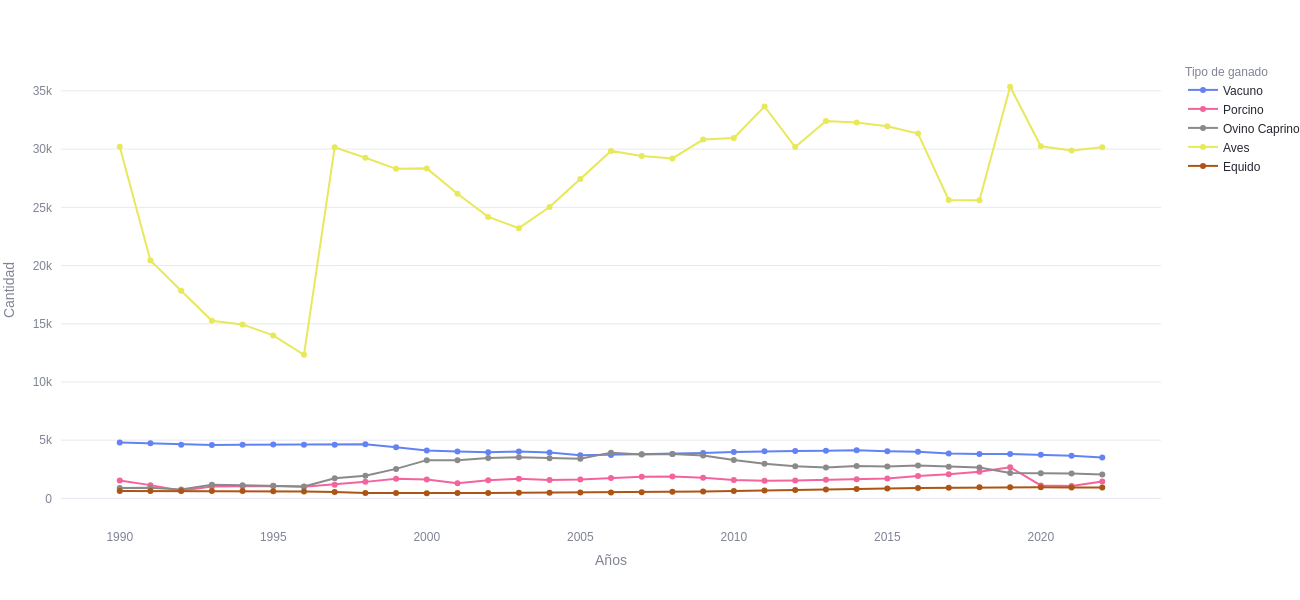
\includegraphics[width=1.0\textwidth]{img/2.1.png}
\end{frame}

\begin{frame}
\begin{block}{Existencia por tipos productores aislados}
    \dots
\end{block}
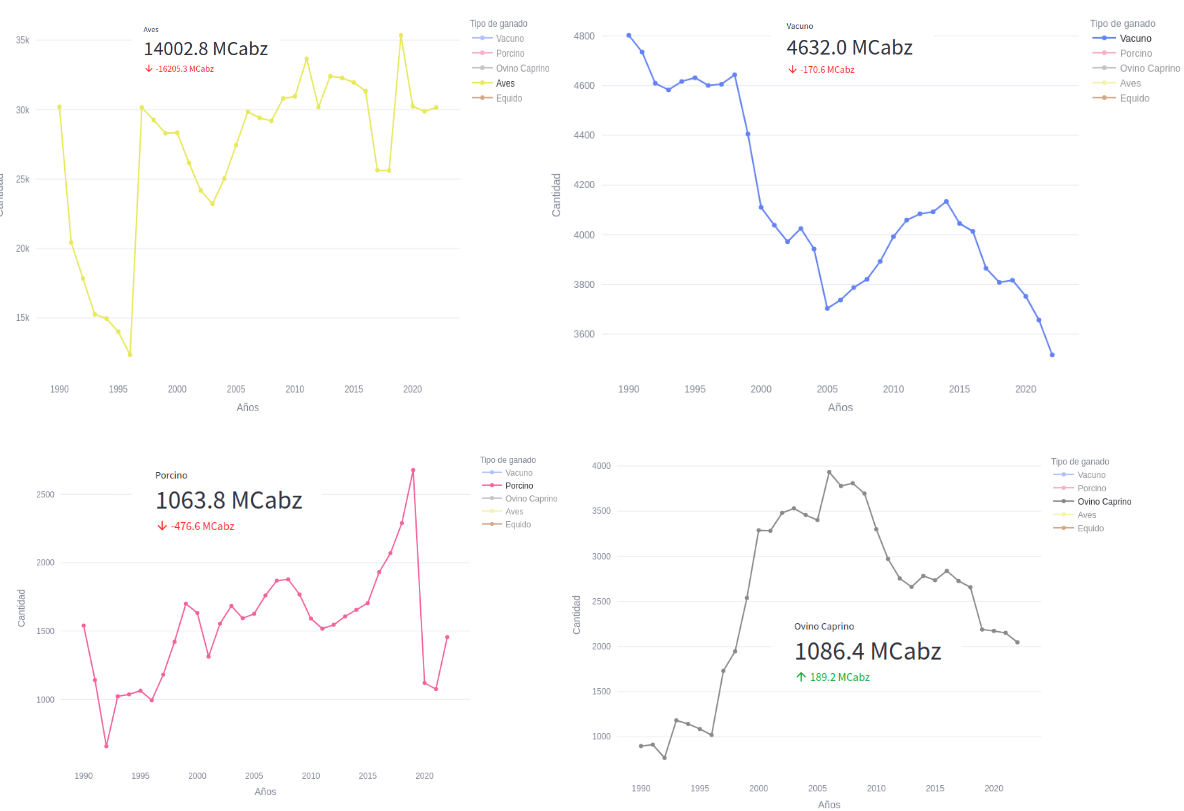
\includegraphics[width=1.0\textwidth]{img/plots_exist.png}
\end{frame}\begin{frame}

\begin{block}{Producción leche}
    \dots
\end{block}
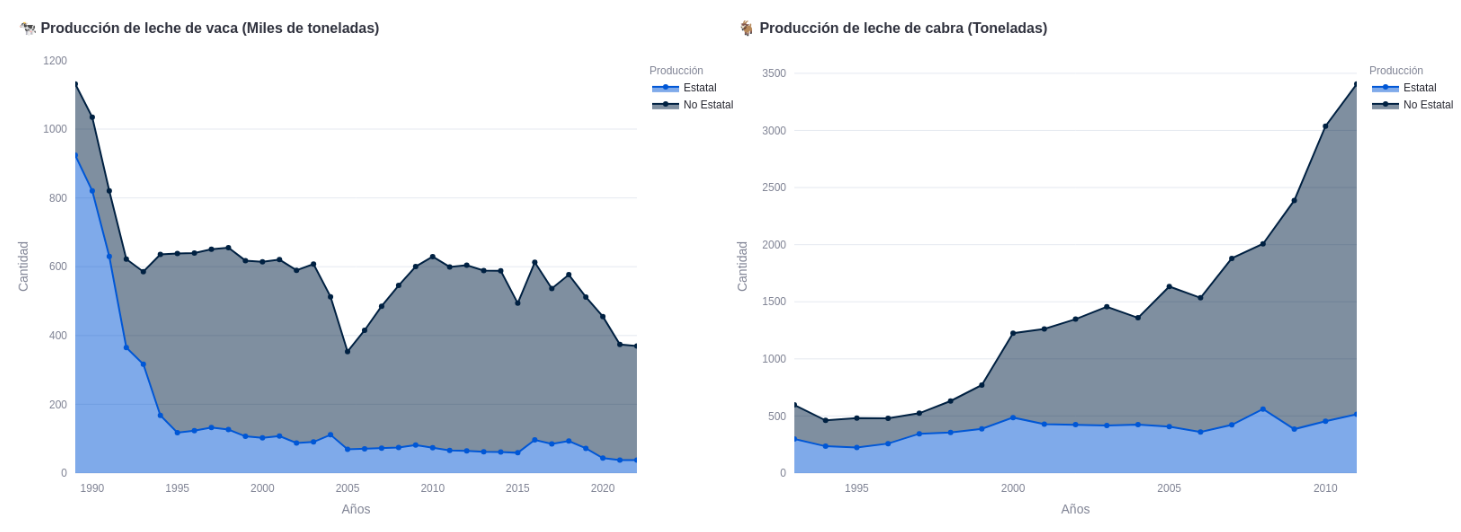
\includegraphics[width=1.0\textwidth]{img/lechee.png}
\end{frame}

\begin{frame}
\begin{block}{Producción de leche por sectores}
    \dots
\end{block}

\includegraphics[width=1.0\textwidth]{img/7.png}

\includegraphics[width=1.0\textwidth]{img/8.png}
\end{frame}

\begin{frame}
\begin{block}{Producción total de huevos}
    \dots
\end{block}
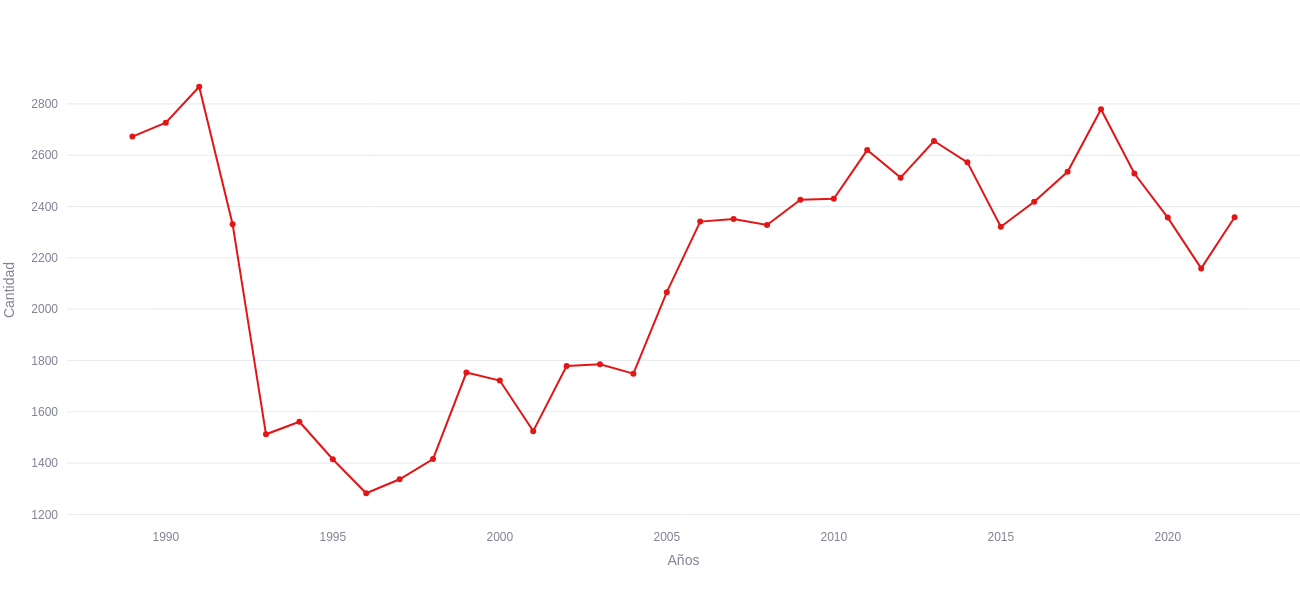
\includegraphics[width=1.0\textwidth]{img/11.png}
\end{frame}

\begin{frame}
\begin{block}{Alimentación}
    \dots
\end{block}
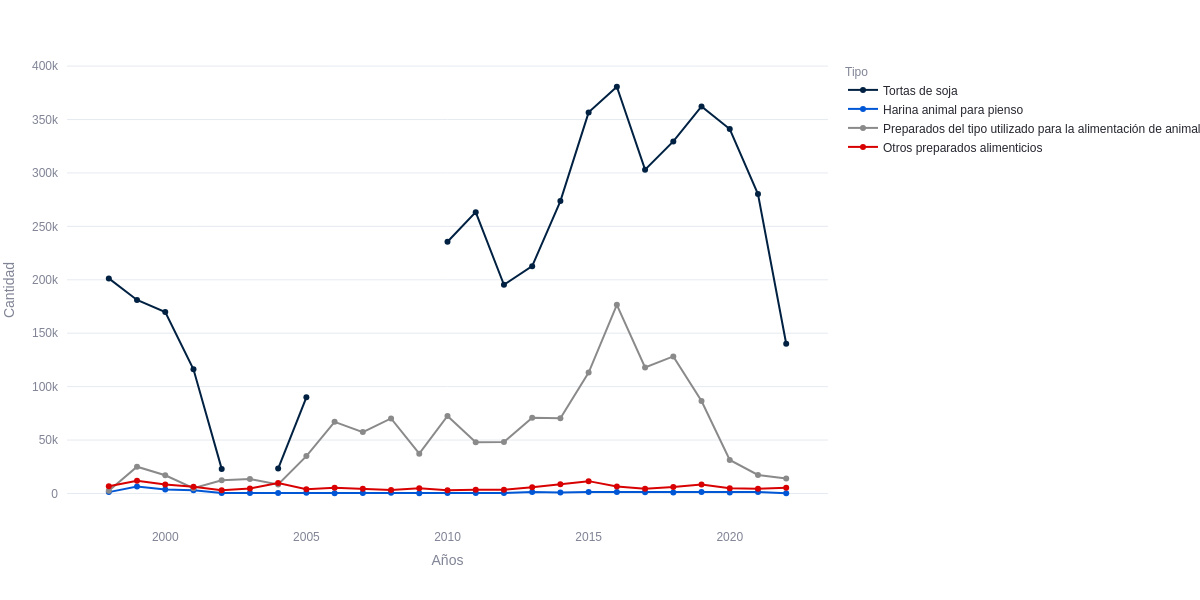
\includegraphics[width=1.0\textwidth]{img/1.png}
\end{frame}

\begin{frame}
\begin{block}{Entidades}
    \dots
\end{block}
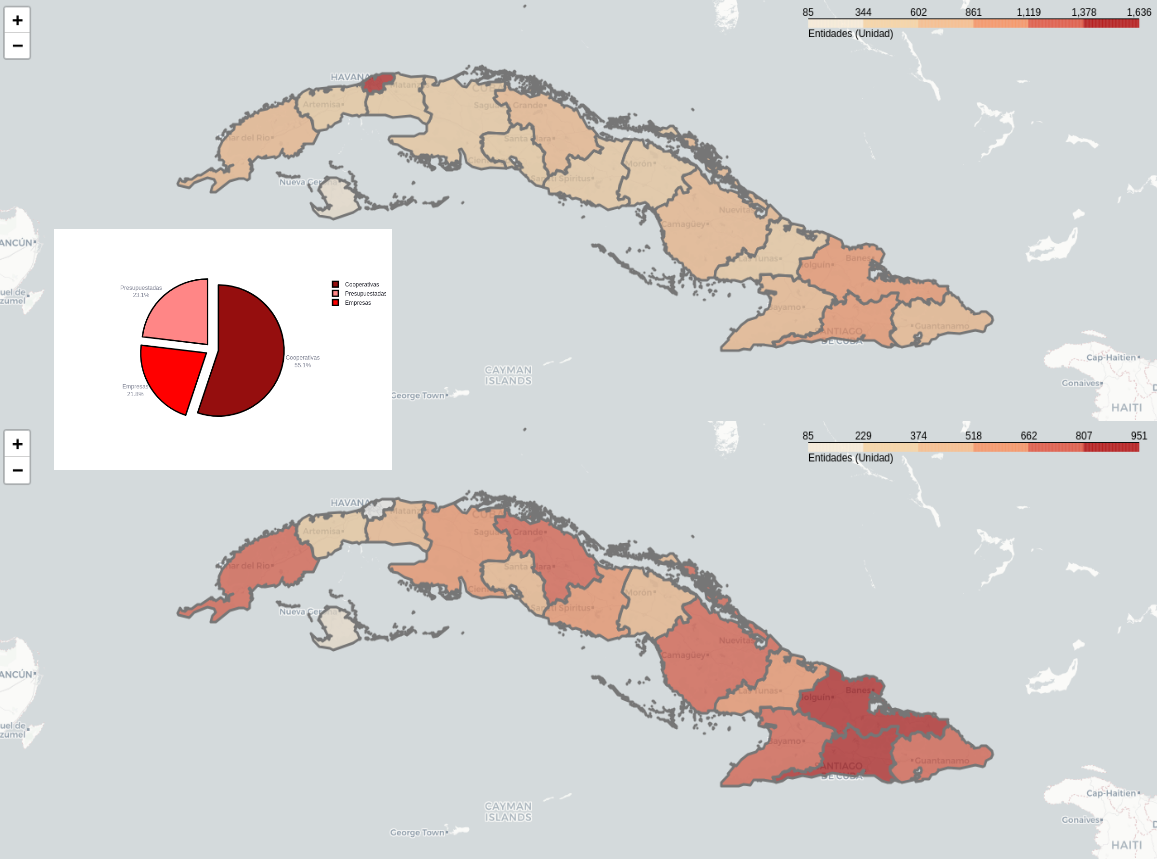
\includegraphics[width=1.0\textwidth]{img/mapa.png}
\end{frame}

\begin{frame}
\begin{block}{Cooperativas}
    \dots
\end{block}
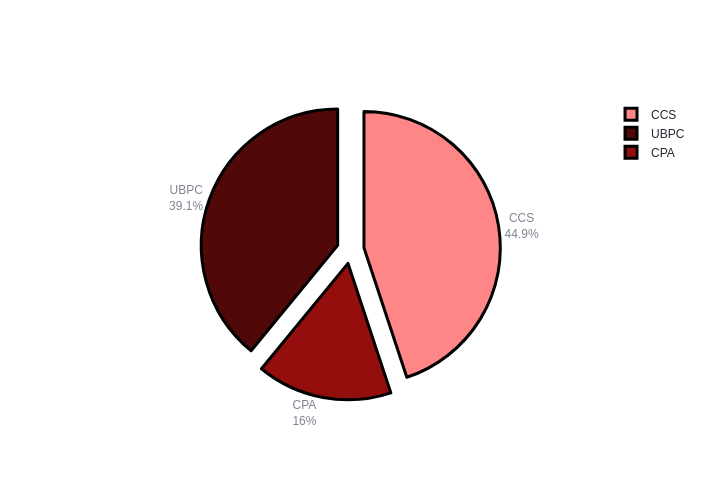
\includegraphics[width=1.0\textwidth]{img/coop.png}
\end{frame}

\section{Historia}
\begin{frame}
\begin{block}{Historia del proceso ganadero cubano}
    \textit{Timeline desde antes del triunfo de la revolución}
\end{block}
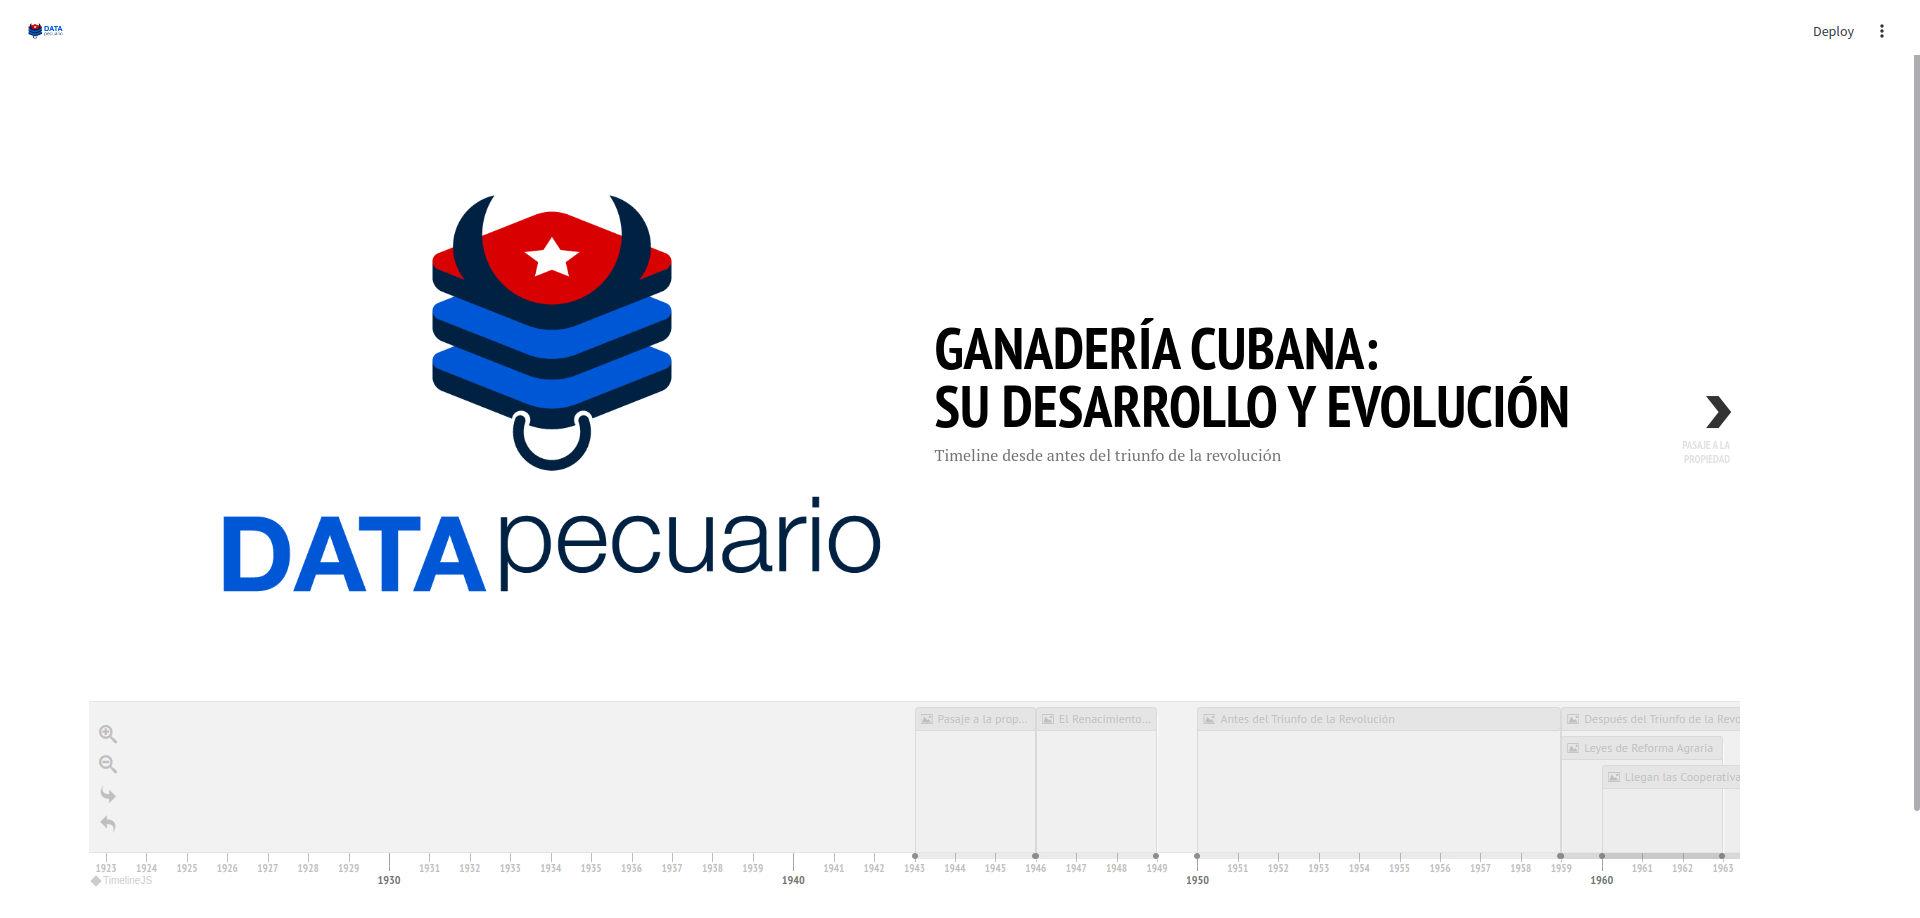
\includegraphics[width=1.0\textwidth]{img/history.png}
\end{frame}

\begin{frame}
\begin{block}{La historia de Luis}
    \dots
\end{block}
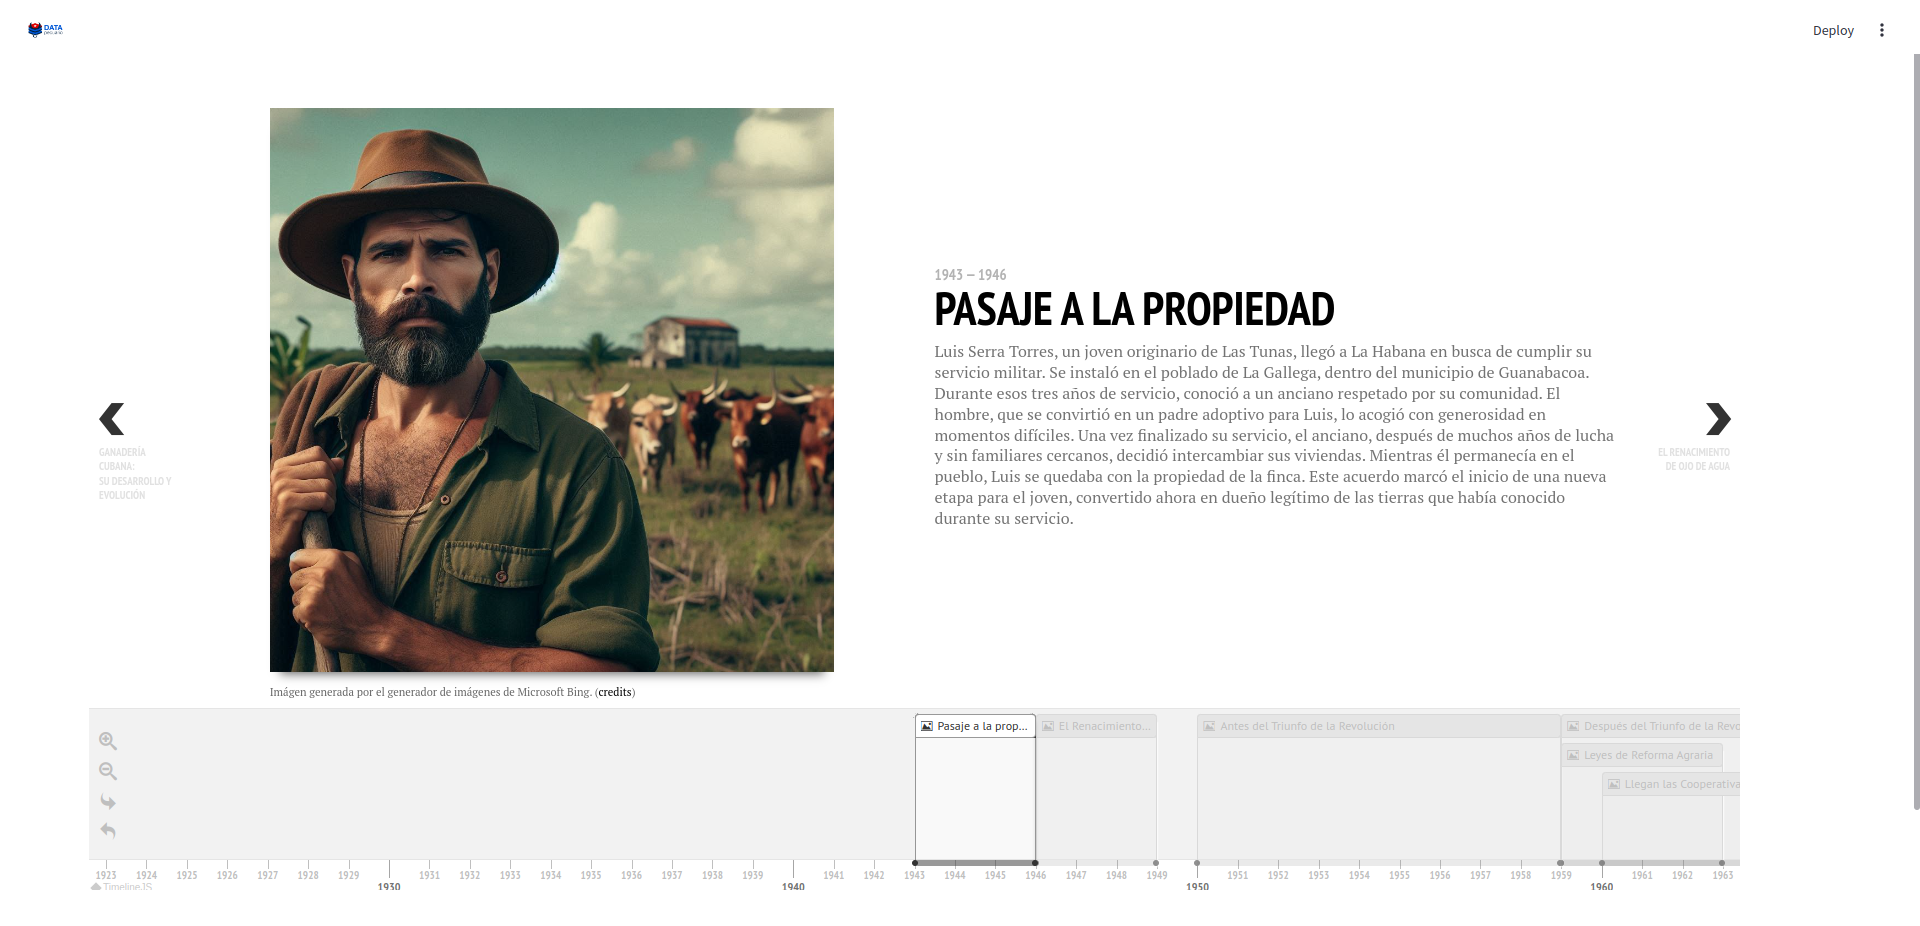
\includegraphics[width=1.0\textwidth]{img/luis.png}
\end{frame}


\begin{frame}
\begin{block}{Podcast RadioPecuario}
\emphh{Temáticas:}
\begin{itemize}
    \item Desafíos generales de la ganadería.
    \item Mejoramiento genético
    \item Alimentación del ganado
\end{itemize}
\textit{Perspectiva del período de la crisis económica de 1990}
\end{block}

\includegraphics[width=1.0\textwidth]{img/web2.png}
\end{frame}


\begin{frame}
\begin{block}{DataPecuario Website}
    \dots
\end{block}
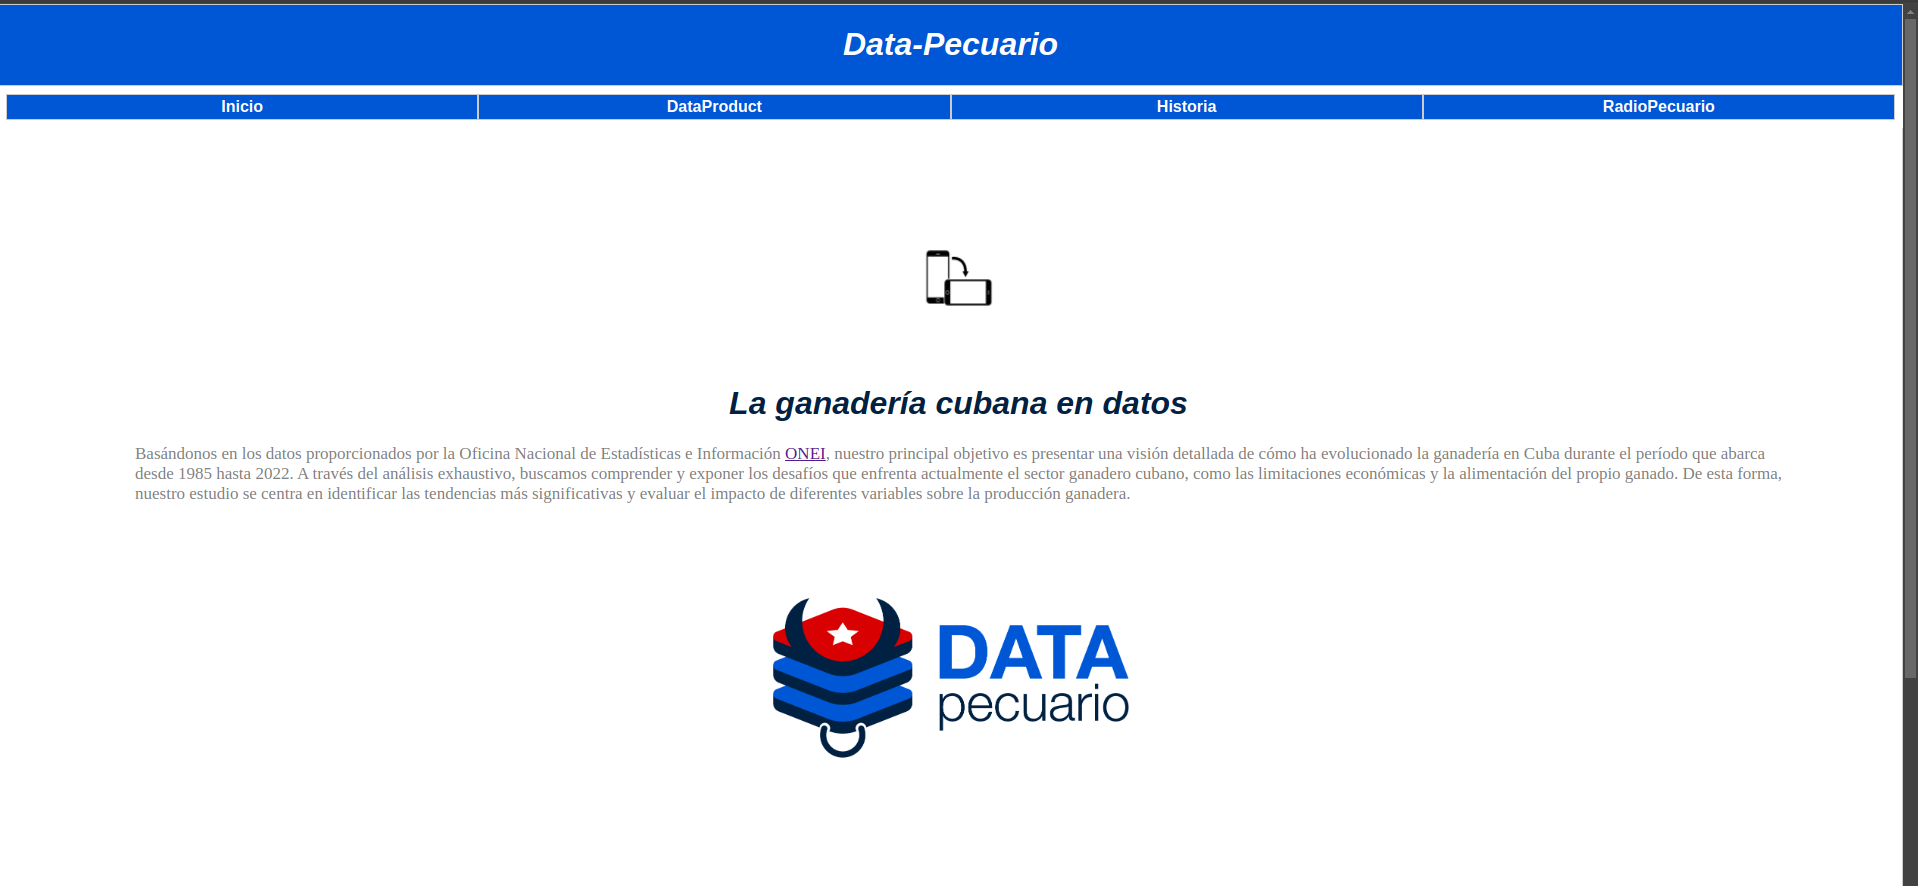
\includegraphics[width=1.0\textwidth]{img/web1.png}
\end{frame}

\begin{section}{Conclusiones}
\begin{frame}
\begin{block}{Conclusiones y recomendaciones}
\begin{itemize}
    \item Dependencia de importaciones
    \item Deficit alimentario
    \item Diversificación de la producción
    \item Inversión en tecnologías y practicas sostenibles
    \item Fomento del desarrollo rural
    \item Mejorar la infraestructura agricola y ganadera
    \item Mayor aprovechamiento de los recursos locales, autosuficiencia alimentaria y una industria ganadera más robusta y competitiva
\end{itemize}
\end{block}
Muchísimas gracias. :)
\end{frame}


\end{document}